\documentclass[]{aastex631}
\usepackage{color}
\usepackage{amsmath}
\usepackage{mathtools,eqparbox}
\usepackage{enumitem}
\usepackage{graphicx}
\usepackage{mathrsfs}
\usepackage{booktabs}
\usepackage{float}
\usepackage{morefloats}
\usepackage{etoolbox}
\usepackage{setspace}
\usepackage{multirow}
\usepackage{longtable}
\usepackage{tikz}
\AtBeginEnvironment{quote}{\par\singlespacing}

\newcommand{\vdag}{(v)^\dagger}
\newcommand\aastex{AAS\TeX}
\newcommand\latex{La\TeX}

\newcommand{\prot}[1]{$P_{{\rm rot} {#1}}$}
\newcommand{\porb}[1]{$P_{{\rm orb} {#1}}$}
\newcommand{\ob}[1]{$\varepsilon_{#1}$}
\newcommand{\ecc}[1]{$e_{#1}$}
\newcommand{\age}{\textsl{age}}
\newcommand{\ttau}[1]{$\tau_{#1}$}
\newcommand{\tq}[1]{$\mathcal{Q}_{#1}$}

\newcommand{\rad}[1]{$R_{#1}$}
\newcommand{\lum}[1]{$L_{#1}$}
\newcommand{\teff}[1]{$T_{\mathrm{eff} {#1}}$}
\newcommand{\logg}{\log g}
\newcommand{\rg}{$r_g$}

\newcommand{\N}[2]{$\mathcal{N}({#1}, {#2})$}
\newcommand{\U}[2]{$\mathcal{U}({#1}, {#2})$}

\newcommand{\mpri}{$M_1$}
\newcommand{\msec}{$M_2$}

\newcommand{\msun}{$M_{\odot}$}
\newcommand{\rsun}{$R_{\odot}$}
\newcommand{\lsun}{$L_{\odot}$}

\definecolor{bcolor}{RGB}{0, 51, 153}
\definecolor{gcolor}{RGB}{10, 100, 10}
\definecolor{dblue}{RGB}{50, 50, 100}
\newcommand{\xxx}[1]{{\color{red}{#1}}}
\newcommand{\remark}[1]{{\color{dblue}{Remark: #1}}}
\newcommand{\todo}[1]{{\color{gcolor}{To do: #1}}}
\newcommand{\code}[1]{{\texttt{#1}}}

\shorttitle{tidal quality factors of binary stars}
\shortauthors{birky et al.}

\graphicspath{{./}{figures/}}

\begin{document}

\title{Theoretical Limits in Constraining Tidal Quality Factors of Binary Stars}


%\correspondingauthor{August Muench}
%\email{greg.schwarz@aas.org, gus.muench@aas.org}

\author{Jessica Birky}
% \affiliation{American Astronomical Society \\
% 1667 K Street NW, Suite 800 \\
% Washington, DC 20006, USA}
\author{Rory Barnes}


\begin{abstract}
\end{abstract}

% \keywords{Classical Novae (251) --- Ultraviolet astronomy(1736) --- History of astronomy(1868) --- Interdisciplinary astronomy(804)}

% ============================================================================
\section{Introduction} \label{sec:intro}

We aim to place theoretical limits on the constraints we can get on \tq\ and \ttau\ using tidal equillibrium models, and disentangle different sources of uncertainty: 
\begin{itemize}
    \item \textbf{Observational:} To what degree is the limitation on the uncertainty of \tq\ and \ttau\ due to a limitation of observational (e.g. ability to observe a parameter, data precision, sample size), which might be improved by better data? That is, how does the accuracy and precision of our observations affect the derived uncertainty of \tq\ and \ttau\, and which observational constraints matter most when it comes to inferring \tq\ and \ttau? What types of systems are most promising for constraining \tq\ and \ttau? Limitation of sample size or limitation of constraints? How do constraints from synchronization (rotation period + eccentricity + orbital period) compare to constraints from circularization (eccentricity + orbital period)? Smaller sample/more constraints vs. larger sample/less constraints

    \item \textbf{Model:} To what degree to inherent degeneracies/pathologies in the model formulation contribute to uncertainty? Is this a problem that is \emph{well posed} for (Bayesian) inference--are the observables sensitive enough to your parameters of interest?

    \item \textbf{Hypothesis:} To what degree does our hypothesis fail to reproduce reality? (comparison between simulated data uncertainties and real data uncertainties; model comparison between CTL, CPL). Can theoretical limits to the uncertainties on \tq\ and \ttau\ derived on \emph{simulated data} give us context to intepret uncertainties on \emph{real data}? Given enough free parameters, it can become possible for a model to reproduce any range of outcomes. How in this situation, can a model be invalidated?
\end{itemize}

% ============================================================================
\section{Methods} \label{sec:methods}

% ----------------------------------------------------------------------------
\subsection{Tidal Evolution Model}

% ----------------------------------------------------------------------------
\subsection{Stellar Evolution + Magnetic Braking Model}

% ----------------------------------------------------------------------------
\subsection{Global Sensitivity Analysis}


% ----------------------------------------------------------------------------
\subsection{Markov Chain Monte Carlo}

% Assumptions for all model experiments:
% \begin{itemize}
% 	\item Both stars in the binary are co-evolutionary and are assumed to have the same age.
% 	\item Tidal quality factors 
% \end{itemize}


\subsection{Observational Constraints}

\textbf{Model initial conditions and observational constraints:} 
\begin{table}[H]
\begin{center}
\begin{tabular}{r|c|c|c|c}
\hline
 			& Model Input 	& Prior & Observational Constraint & Good Unc \\
\hline
 \mpri\			& primary mass [\msun] 				& \N{m}{s} 			& kepler solution (lc eclipse + rvs) & 0.001 \\   
 \msec\			& secondary mass [\msun]			& \N{m}{s} 			& kepler solution (lc eclipse + rvs) & 0.001 \\     
 \prot{1,i}  	& pri init rotation period [days]	& $log$\N{m}{s}		& dist in young open clusters & 		\\ 
 \prot{2,i}  	& sec init rotation period [days]	& $log$\N{m}{s}		& dist in young open clusters & 		\\   
 \porb{,i}		& init orbital period [days]		& \U{4.0}{10.0} 	& uninformed 			  & 		\\ 
 \ecc{i}		& init eccentricity 				&  \U{0}{0.5}		& uninformed 			& 		\\  
 \age\			& system age [yr]					&  \N{m}{s} 		& open cluster age 			& 	10\%	\\
 \ob{1,i}		& pri init obliquity [deg]			&   \U{0}{30}		& uninformed 						  & 		\\ 
 \ob{2,i}		& sec init obliquity [deg]			& 	\U{0}{30}		& uninformed 						  & 		\\ 
\hline
 \tq{1}			& pri tidal phase lag  & 	\U{4}{9}	& uninformed 						  & 		\\ 
 \tq{2}			& sec tidal phase lag  & 	\U{4}{9}	& uninformed 						  & 		\\ 
\hline
 \ttau{1}		& pri tidal time lag [log(s)]  & 	\U{-4}{2}	& uninformed 						  & 		\\ 
 \ttau{2}		& sec tidal time lag [log(s)] & 	\U{-4}{2}	& uninformed 						  & 		\\ 
\hline
\end{tabular}
\end{center}
\end{table}

\textbf{Model final conditions and observational constraints:} 
\begin{table}[H]
\begin{center}
\begin{tabular}{r|c|c|c|c}
\hline
 			& Model Output 	& Likelihood & Observational Constraint & Good Unc \\
\hline
 \prot{1,f}  	& pri final rotation period [days]	& \N{m}{s}		& lc autocorrelation function  & 	0.1	\\ 
 \prot{2,f}  	& sec final rotation period [days]	& \N{m}{s}		& spectroscopic $v\sin i$  & 	0.1	\\   
 \porb{,f}		& final orbital period [days]		& \N{m}{s}		& lc lomb scargle			  & $10^{-5}$		\\ 
 \ecc{f}		& final eccentricity 				& \N{m}{s}		& lc eclipse + rvs 			& 	0.001	\\      
\hline
 \rad{1,f}		& pri final radius [\rsun]			& \N{m}{s}		& stellar models + photometry			& 	0.01	\\ 
 \rad{2,f}		& sec final radius [\rsun]			& \N{m}{s}		& eclipse shape	+ pri radius		& 	0.01	\\
 \lum{1,f}		& pri final lumniosity [\lsun]		& \N{m}{s}		& stellar models + photometry			& 	0.1	\\ 
 \lum{2,f}		& sec final lumniosity [\lsun]		& \N{m}{s}		& stellar models + photometry		& 	0.1	\\
 \teff{1,f}		& pri final temperature [K]			& \N{m}{s}		& stellar models + spectra			& 	\\ 
 \teff{2,f}		& sec final temperature [K]			& \N{m}{s}		& stellar models + spectra		& 	\\
\hline
\end{tabular}
\end{center}
\end{table}



% ============================================================================
\section{Results} \label{sec:results}

\begin{itemize}
	\item sensitivity analysis (full 9 parameters + age) - CTL, CPL, CTL + STELLAR, CPL + STELLAR
		\subitem free parameters: \mpri, \msec, \ob{1,i}, \ob{2,i}, \prot{1,i}, \prot{2,i}, \ecc{i}, \porb{,i}, \tq\
		\subitem computation time: $\sim$30 min eqtide only, $\sim$1 day for eqtide + stellar
	\item sensitivity analysis (6 parameters + age) - CTL, CPL, CTL + STELLAR, CPL + STELLAR
		\subitem free parameters: \mpri, \msec, \prot{1,i}, \prot{2,i}, \ecc{i}, \tq\ (without obliquity, prior for porb based on final porb, ecc)
		\subitem computation time: $\sim$30 min eqtide only, $\sim$1 day for eqtide + stellar
	\item MCMC recovery test on synthetic data (4 parameters + age)
		\subitem free parameters: \prot{1,i}, \prot{2,i}, \ecc{i}, \tq\ (fix masses, without obliquity, prior for porb based on final porb, ecc)
		\subitem computation time (per MCMC run): $\sim$ few hours for eqtide only, $\sim$ few weeks for eqtide + stellar
	\item 1D likelihood tests
		\subitem free parameters: \tq\
		% \subitem have tried running mcmc sampling on 1D likelihood functions, but dynesty is unable to sample--returns error that likelihood is too flat
	\item MCMC recovery test on real data (4 parameters + age)?
		\subitem if there's an open cluster system in a tide-sensitive age range
		\subitem comparison with the synthetic data tests may be able to tell us how much posterior uncertainty is due to which input parameters/observational uncertainties/degeneracies?
\end{itemize}

\begin{figure}[ht!]
\begin{center}
	\caption{EQTIDE + STELLAR: CPL model}
	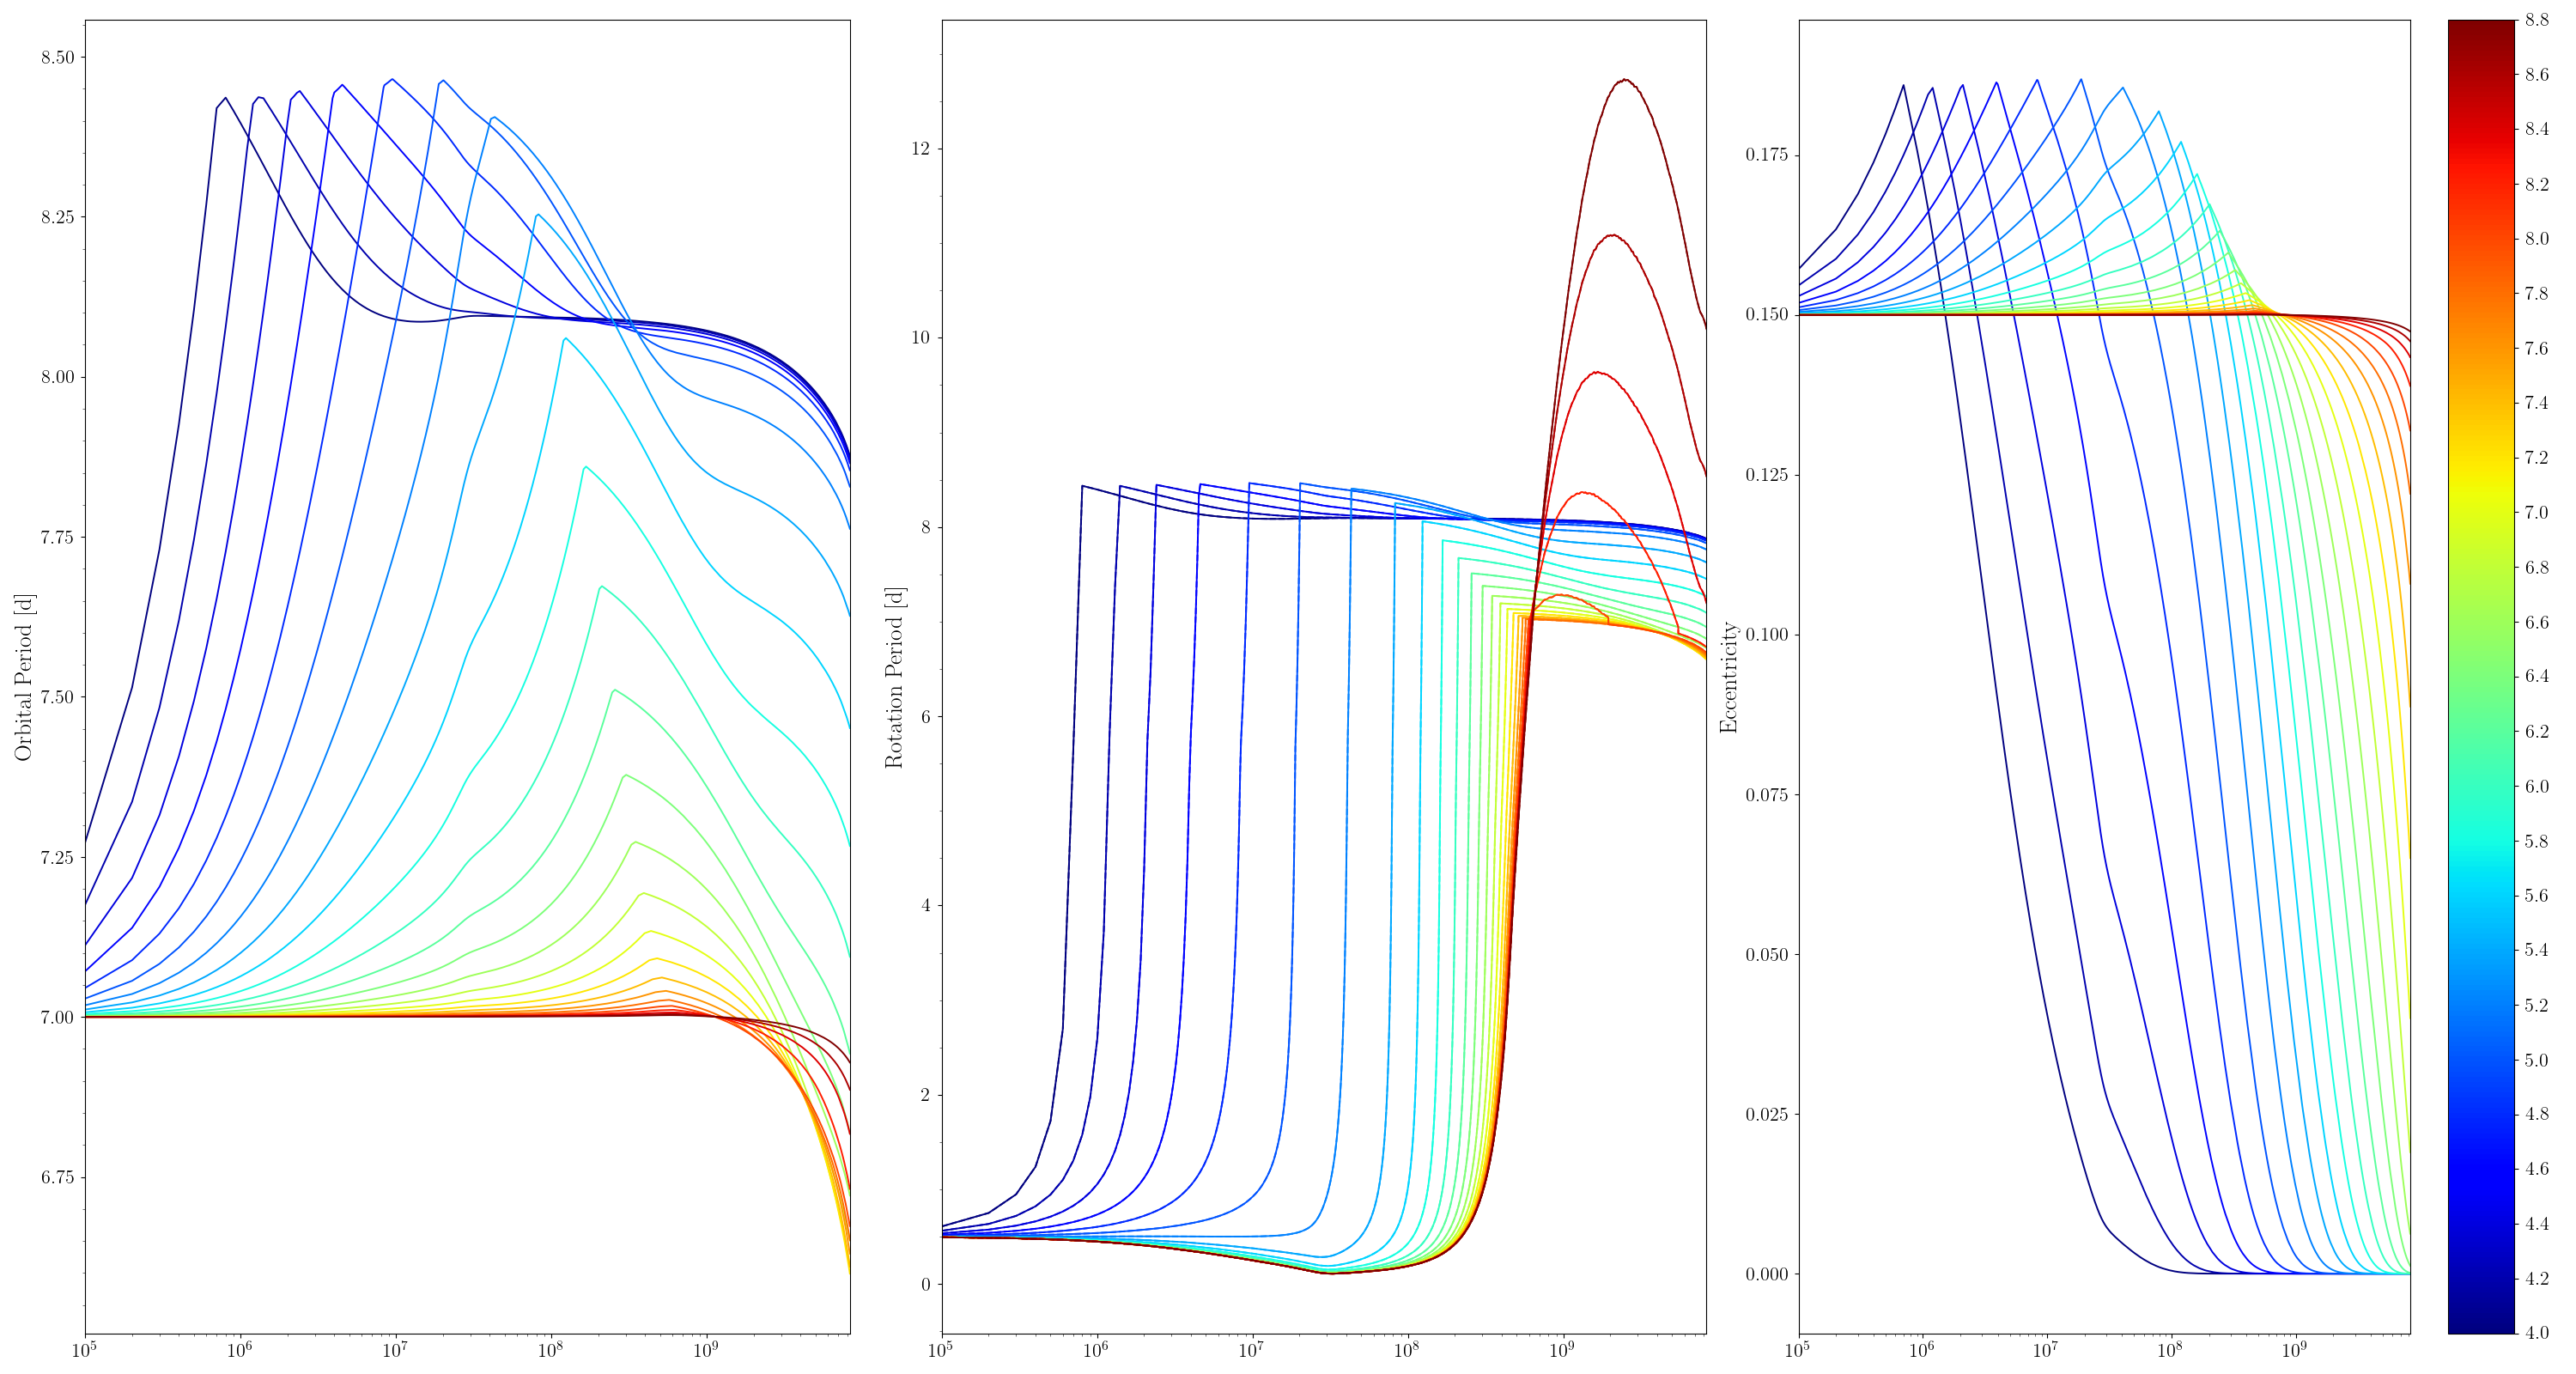
\includegraphics[width=\linewidth]{../analysis/results_likelihood_1d/cpl_stellar_eqtide/plots/vary_q_evolution.png} 
	\caption{EQTIDE + STELLAR: CTL model}
	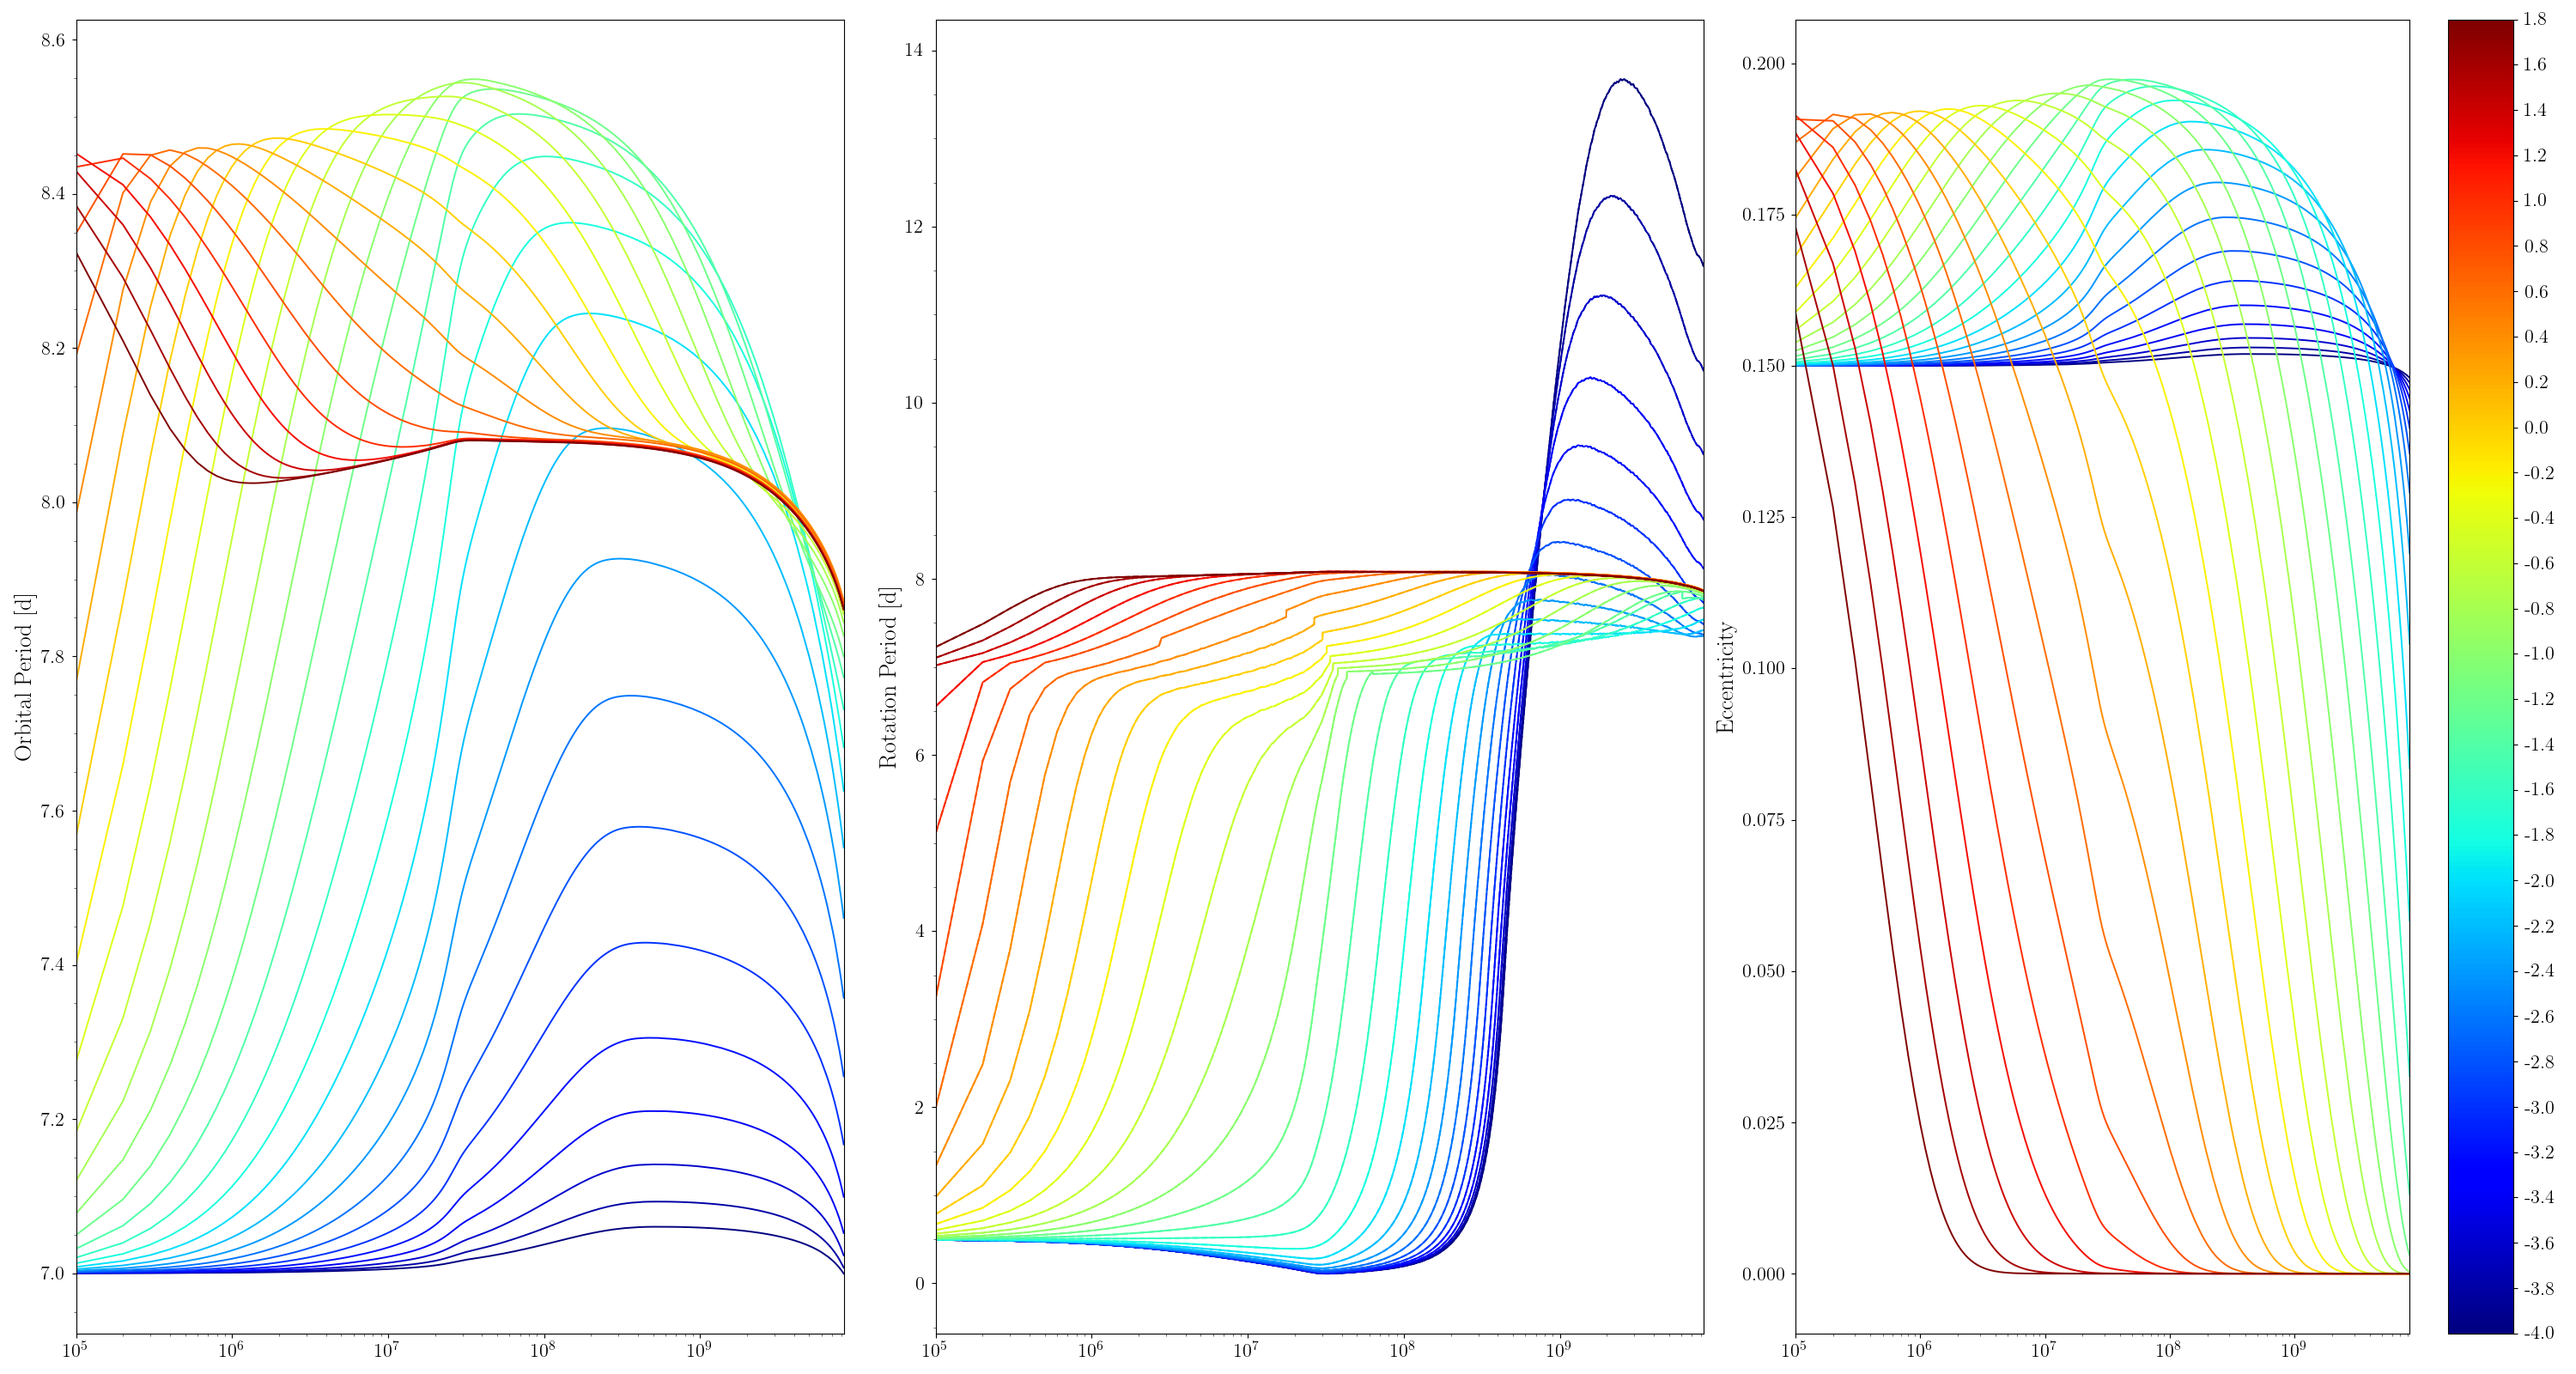
\includegraphics[width=\linewidth]{../analysis/results_likelihood_1d/ctl_stellar_eqtide/plots/vary_tau_evolution.png} 
\end{center}
\end{figure}

\begin{figure}[ht!]
\begin{center}
	% \caption{CTL model (top) and CPL model (bottom)}
	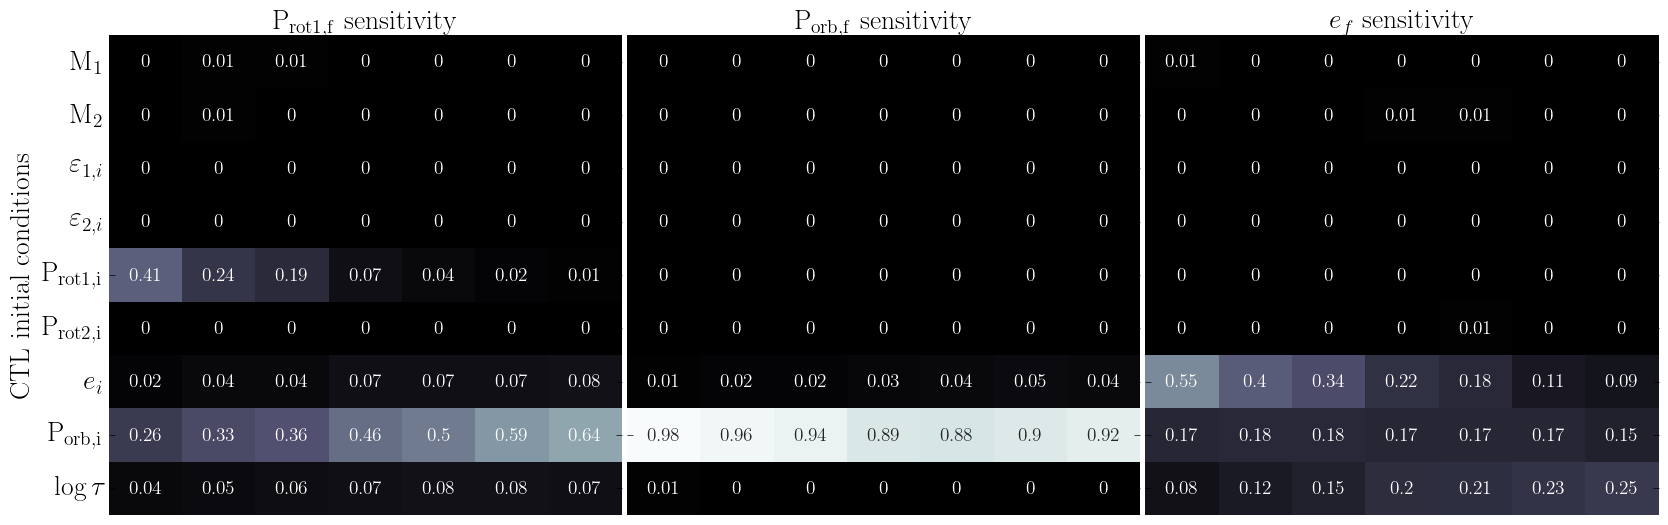
\includegraphics[width=\linewidth]{../figures/sensitivity_ctl.png} 
	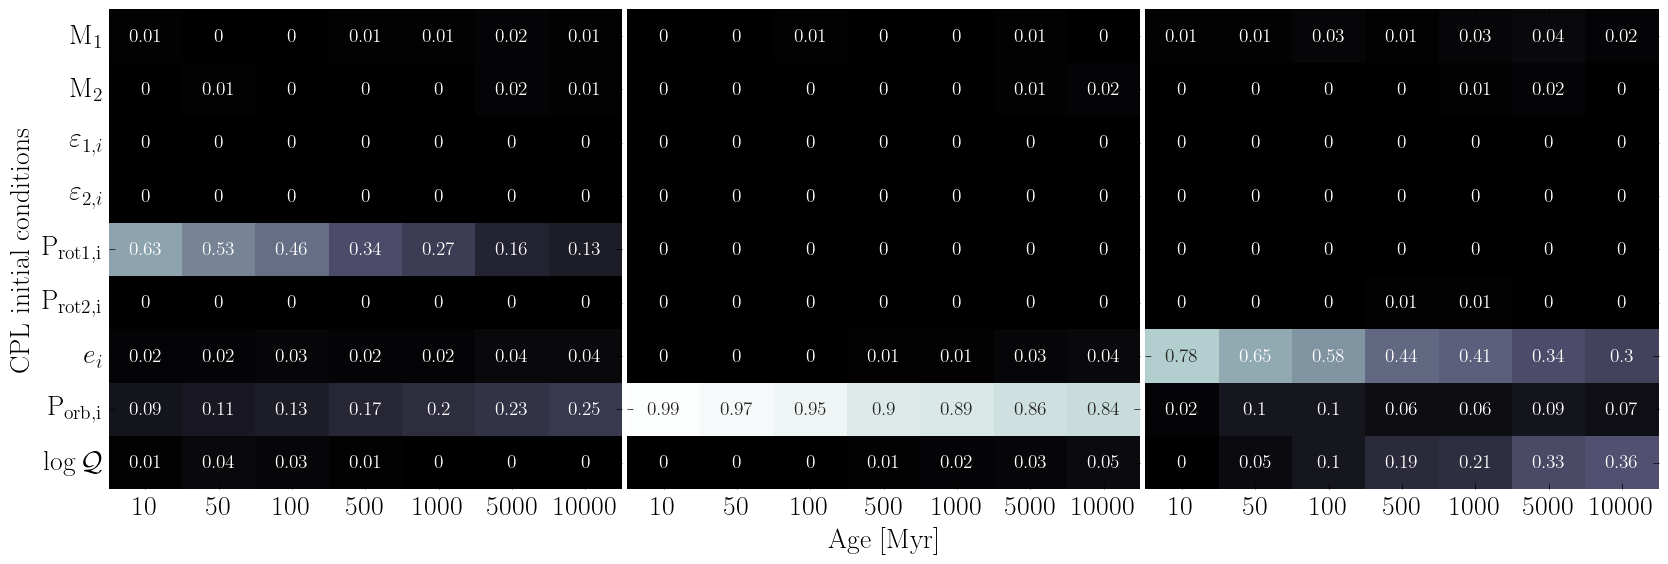
\includegraphics[width=\linewidth]{../figures/sensitivity_cpl.png}
\end{center}
\end{figure}

\begin{figure}[ht!]
\begin{center}
	% \caption{CTL model (top) and CPL model (bottom)}
	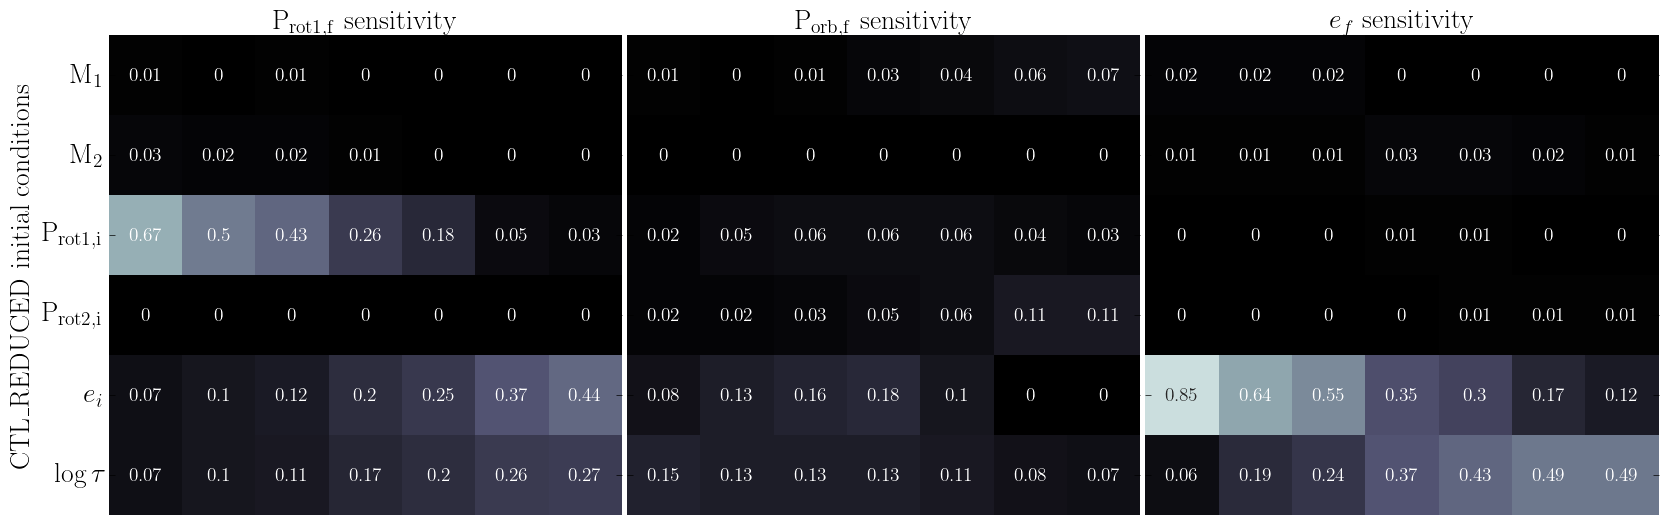
\includegraphics[width=\linewidth]{../figures/sensitivity_ctl_reduced.png} 
	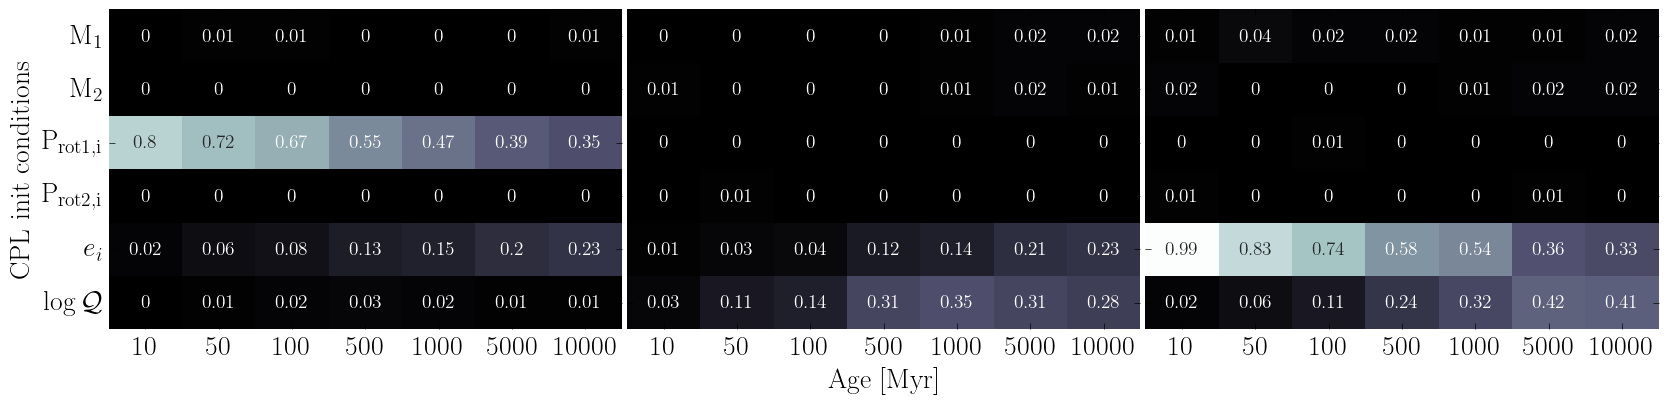
\includegraphics[width=\linewidth]{../figures/sensitivity_cpl_reduced.png}
\end{center}
\end{figure}

% ============================================================================
\section{Discussion} \label{sec:discusstion}



% ============================================================================
\section{Conclusion} \label{sec:conclusion}


\hfill \break % ============================================================================
% \begin{appendix} \label{sec:appendix}
\newpage
\appendix \label{sec:appendix}


% ============================================================================
% \newpage
\bibliography{ref}{}
\bibliographystyle{aasjournal}

\end{document}